El análisis que se realiza de los resultados obtenidos es comparando la calidad de los resultados de los algoritmos discutidos en la sección desarrollo, sobre las bases de datos de la sección búsqueda. Con el objetivo de evaluar las propuestas algorítmicas, se consideraron los siguientes métodos:

\begin{itemize}
\item{$alg1$} PAC(C-HAC / selección simple)
\item{$alg2$} PAC(BOBO-10 / selección simple)
\item{$alg3$} PAC(BOBO-10 / selección proporcional)
\item{$alg4$} PAC(BOBO-10 / selección proporcional) + tabú
\item{$alg5$} PAC(Intra-Inter C-HAC / selección proporcional)
\item{$alg6$} PAC(Intra-Inter C-HAC / selección proporcional) + tabú
\item{$alg7$} Construcción golosa
\item{$alg8$} Construcción golosa + tabú
\end{itemize}

Para la experimentación se utilizó una máquina Desktop Intel(R) Core(TM) i5-4570T CPU @ 2.90GHz, 5.7G Ram, con DB: 5.5.46-MariaDB-1ubuntu0.14.04.2.

Tanto $alg1$ como $alg2$ corresponden a metodologías propuestas en \cite{compositeRetrival}. Los otros algoritmos involucran las mejoras propuestas en este trabajo, para PAC es Intra-Inter C-HAC en la etapa de producción y la selección proporcional en la etapa de selección. En los casos que se agregá la búsqueda tabú, En \texttt{PAC} se realiza la búsqueda tabú \texttt{Inter-Paquete} luego de la etapa de producción y la \texttt{Intra-Paquete} luego de la selección. En la \texttt{Búsqueda Golosa} de la solución obtenida se realiza la búsqueda tabú \texttt{Intra-Paquete}. Cabe señalar que no se tienen en consideración BOBO-Ex y CAP ya que para el tamaño de la instancia los tiempos de ejecución de esos algoritmos resultaron prohibitivos. A partir de experimentación preliminar con BOBO para valores $c=1, 5$ y $10$, resultó $c=10$ la opción más competitiva.  Para la búsquedas tabú se definió que la cantidad de iteraciones de permanencia de un elemento en la lista tabú sea el promedio de elementos que tiene un paquete en la solución inicial.

Para realizar una comparación entre la calidad de las soluciones obtenidas por los diferentes algoritmos, se ha evaluado para los $\gamma \in \left\{0,1; 0,3; 0,4; 0,5; 0,6; 0,7; 0,8; 0,9\right\} $el porcentaje de deterioro de cada solución.

En el caso de la búsqueda de artículos, que es el escenario que contiene la mayor cantidad de objetos, los tiempos de ejecución  para los algoritmos C-HAC ($alg1$, $algo5$ y $alg6$) son del orden de los 5 minutos, mientras que para los algoritmos BOBO ($alg2$, $alg3$ y $alg4$) de 2 minutos y los golosos ($alg7$ y $alg8$) de los x minutos. Los incrementos de tiempo debido a la ejecución de las metaheruísticas de mejora son despreciables, están entre los 5 y 7 segundos. Por lo cual no se considera que el tiempo sea un factor que valga la pena analizar.

\section{Base de datos de artículos}
Para optimizar el tiempo de consulta de la similitud entre dos objetos, se tiene en memoria una matriz con todos los valores de la función similitud. En consecuencia aumenta la complejidad espacial, en las consultas que se realizaron en este trabajo la instancia utilizada no contiene más de $7000$ elementos por lo que la matriz de similitud no supera los $2$ GB de memoria. Por lo tanto, en este caso, es favorable utilizar la matriz.

Para comprender el comportamiento de los resultados de las búsquedas se diseñaron dos tipos de gráficos que permiten visualizar de la solución la cohesión de los paquetes y la distancia entre ellos. De esta forma se podrá analizar la calidad del resultado obtenido más allá del valor de la función objetivo.

Los gráficos del estilo de \ref{res:img-explain-bars} permiten concluir la distribución de los tópicos de una solución a nivel de paquete y de la relación con otros. En los que se visualiza a través del tamaño del círculo la proporción del artículo con el tópico y el color hace referencia al paquete que el artículo pertenece. Por lo tanto si para un paquete se tiene que la distribución entre los tópicos y el tamaño de los círculos es similar para cada artículo se puede deducir que ese paquete es cohesivo. Por otro lado si el tamaño de los círculos de un paquete no coinciden con los de otro paquete indica que el resultado es diverso.
\begin{figure}[H]
  \centering
    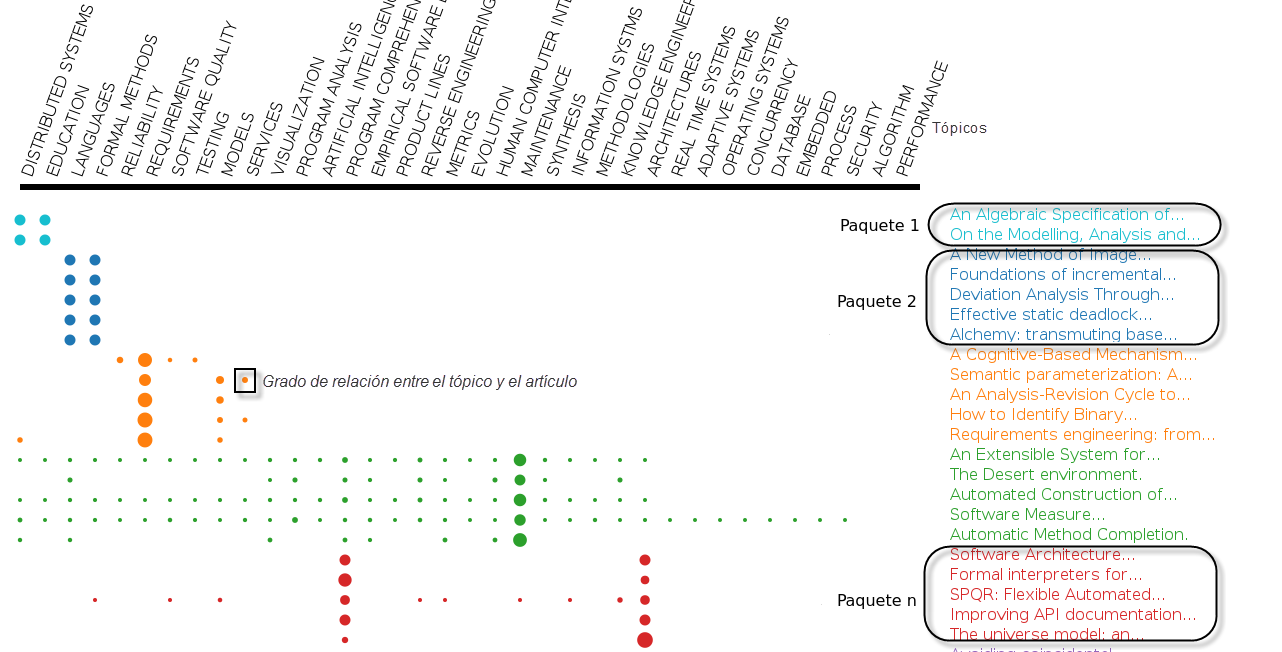
\includegraphics[width=1\textwidth]{img/explain-bars.png}
  \caption{}
  \label{res:img-explain-bars}
\end{figure}

Los gráficos de tipo burbuja \ref{res:img-explain-bubbles} son utiles para concluir el nivel de acoplamiento entre los paquetes de una solución, observando la relación entre los tópicos y los paquetes. Cada burbuja representa un tópico que contiene círculos; cada circulo es un artículo donde el tamaño es la proporción del articulo con el tópico y el color el paquete al que pertenece. Entonces si las burbujas contienen círculos de más de un color se puede decir que ese resultado no es muy diverso, mientras que el color de los círculos de las burbujas sea más homogéneo el resultado es más diverso. En cuanto a la cohesión de los paquetes, es más cohesivo cuando el tamaño de cada circulo dentro de cada burbuja sea similar (para el mismo color) y la distribución de los círculos entre cada burbuja es equitativa.

\begin{figure}[H]
  \centering
    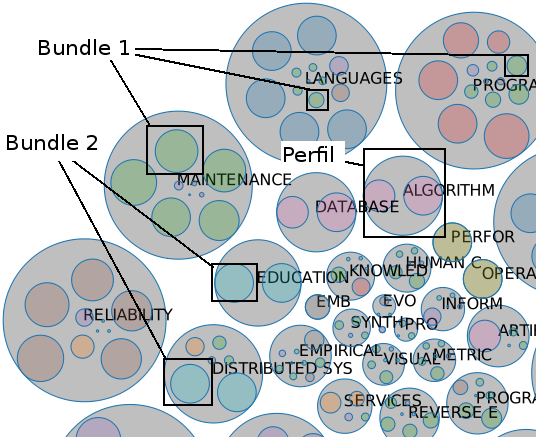
\includegraphics[width=0.5\textwidth]{img/explain-bubbles.png}
  \caption{}
  \label{res:img-explain-bubbles}
\end{figure}

En la tabla \ref{tabla:comp1} se observa los porcentajes de deterioro. Una primera observación es que los algoritmos  Intra-Inter C-HAC reflejan el efecto buscado: a menores valores de $\gamma$ donde el valor inter tiene mayor peso, se obtienen mejores soluciones. Es decir, haber considerado en el proceso de generación de paquetes la funcion Intra-Inter benefició a la calidad de las soluciones obtenidas. Claramente, a medida que $\gamma$ crece y la función intra adquiere mayor preponderancia, la función $Score$ tiene mejor performance. Los algoritmos BOBO, no obtienen soluciones de la calidad de los algoritmos C-HAC y el proceso de selección proporcional no logra una mejora consistente para todos los valores de $\gamma$. Las soluciones obtenidas con el algoritmo de construcción golosa, no alcanzaron a mejorar las soluciones de C-HAC pero fueron ampliamente mejores que las de BOBO. En promedio el porcentaje de deterioro de BOBO fue de un $50\%$ mientras que el goloso fue de un $12\%$. 
Cabe resaltar el muy buen rendimiento de la búsqueda tabú, tanto en escenarios donde la solución inicial no es de buena calidad (algoritmo BOBO) así como también considerando soluciones de mejor calidad (algoritmo Intra-Inter C-HAC). En el primer caso, se obtienen porcentajes de mejora por encima del $70\%$. En el segundo caso, para varios valores de $\gamma$ la solución obtenida por la búsqueda tabú resultó ser la mejor opción y en otros con deterioros inferiores al $0.5\%$.
\begin{table}
\begin{center}
\begin{tabular}{|c|c|c|c|c|c|c|c|c|}
\hline
$\gamma$&$alg1$&$alg2$&$alg3$&$alg4$&$alg5$&$alg6$&$alg7$&$alg8$ \\ \hline
0.1 & -2.34	& -35.06 & -37.11 & -13.48 & -0.72 &  0.00 &  -4.82 &  -4.38 \\
0.2 & -2.45	& -40.01 & -40.05 & -6.28 & -0.35 &  0.00 &  -5.25 &  -4.46 \\
0.3 & -3.39	& -44.54 & -44.50 & -11.63 & -1.10 &  0.00 & -10.16 &  -9.09 \\
0.4 & -0.45	& -48.85 & -50.16 & -3.00 & -0.31 &  0.00 & -10.68 &  -9.95 \\
0.5 & 0.00  & -52.32 & -52.62 & -7.38 & -0.31 & -0.02 & -12.97 & -12.07 \\
0.6 & -0.19 & -55.57 & -54.98 & -6.83 & -0.24 &  0.00 & -14.94 & -13.97 \\
0.7 & 0.00  & -57.11 & -56.52 & -9.36 & -0.41 & -0.21 & -16.21 & -15.19 \\
0.8 & 0.00  & -57.90 & -57.83 & -6.08 & -0.56 & -0.41 & -18.10 & -16.99 \\
0.9 & 0.00  & -58.51 & -58.44 & -6.41 & -0.48 & -0.23 & -20.47 & -19.31 \\ \hline 
\end{tabular}
\caption{Comparaci\'on de calidad de soluciones entre algoritmos} 
\label{tabla:comp1}
\end{center}
\end{table}

En los gráficos \ref{res:img-papers-agr-gamma01} y \ref{res:img-papers-agr-gamma09} se muestran agrupados por algoritmo de resolución las diferentes estrategias usadas en cada caso y los valores de la función objetivo alcanzado toma los dos extremos del valor de $\gamma$ $0.1$ y $0.9$. La recta horizontal es la cota máxima para la función objetivo según la instancia del problema.

\begin{figure}[H]
  \centering
    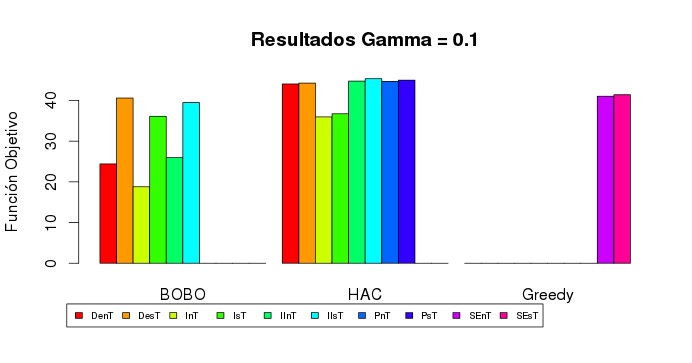
\includegraphics[width=0.8\textwidth]{resultados/papers/Graficos_agrupados/gamma01.png}
  \caption{Función Objetivo $\gamma$ = $0.1$ vs Algoritmos de resolución}
  \label{res:img-papers-agr-gamma01}
\end{figure}

\begin{figure}[H]
  \centering
    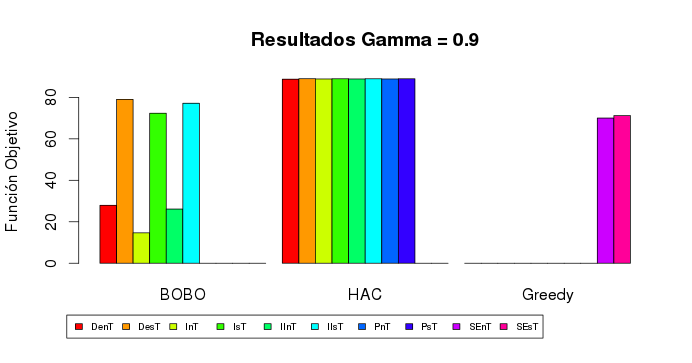
\includegraphics[width=0.8\textwidth]{resultados/papers/Graficos_agrupados/gamma09.png}
  \caption{Función Objetivo $\gamma$ = $0.9$ vs Algoritmos de resolución}
  \label{res:img-papers-agr-gamma09}
\end{figure}

De lo anterior se observa que para todos valores de $\gamma$ las soluciones obtenidas al aplicar la búsqueda tabú se mejora la función objetivo, en el caso de BOBO la mejora es más significativa que en los otros.\\

\paragraph{Jerárquico (Efficient C-HAC)}
En \ref{res:img-papers-agr-gamma01} y \ref{res:img-papers-agr-gamma09} se visualiza que utilizando la búsqueda Tabú al final de la ejecución de HAC no mejora considerablemente la solución. Por lo que se decidió para este caso comparar el algoritmo sin la búsqueda tabú.
\begin{figure}[H]
  \centering
    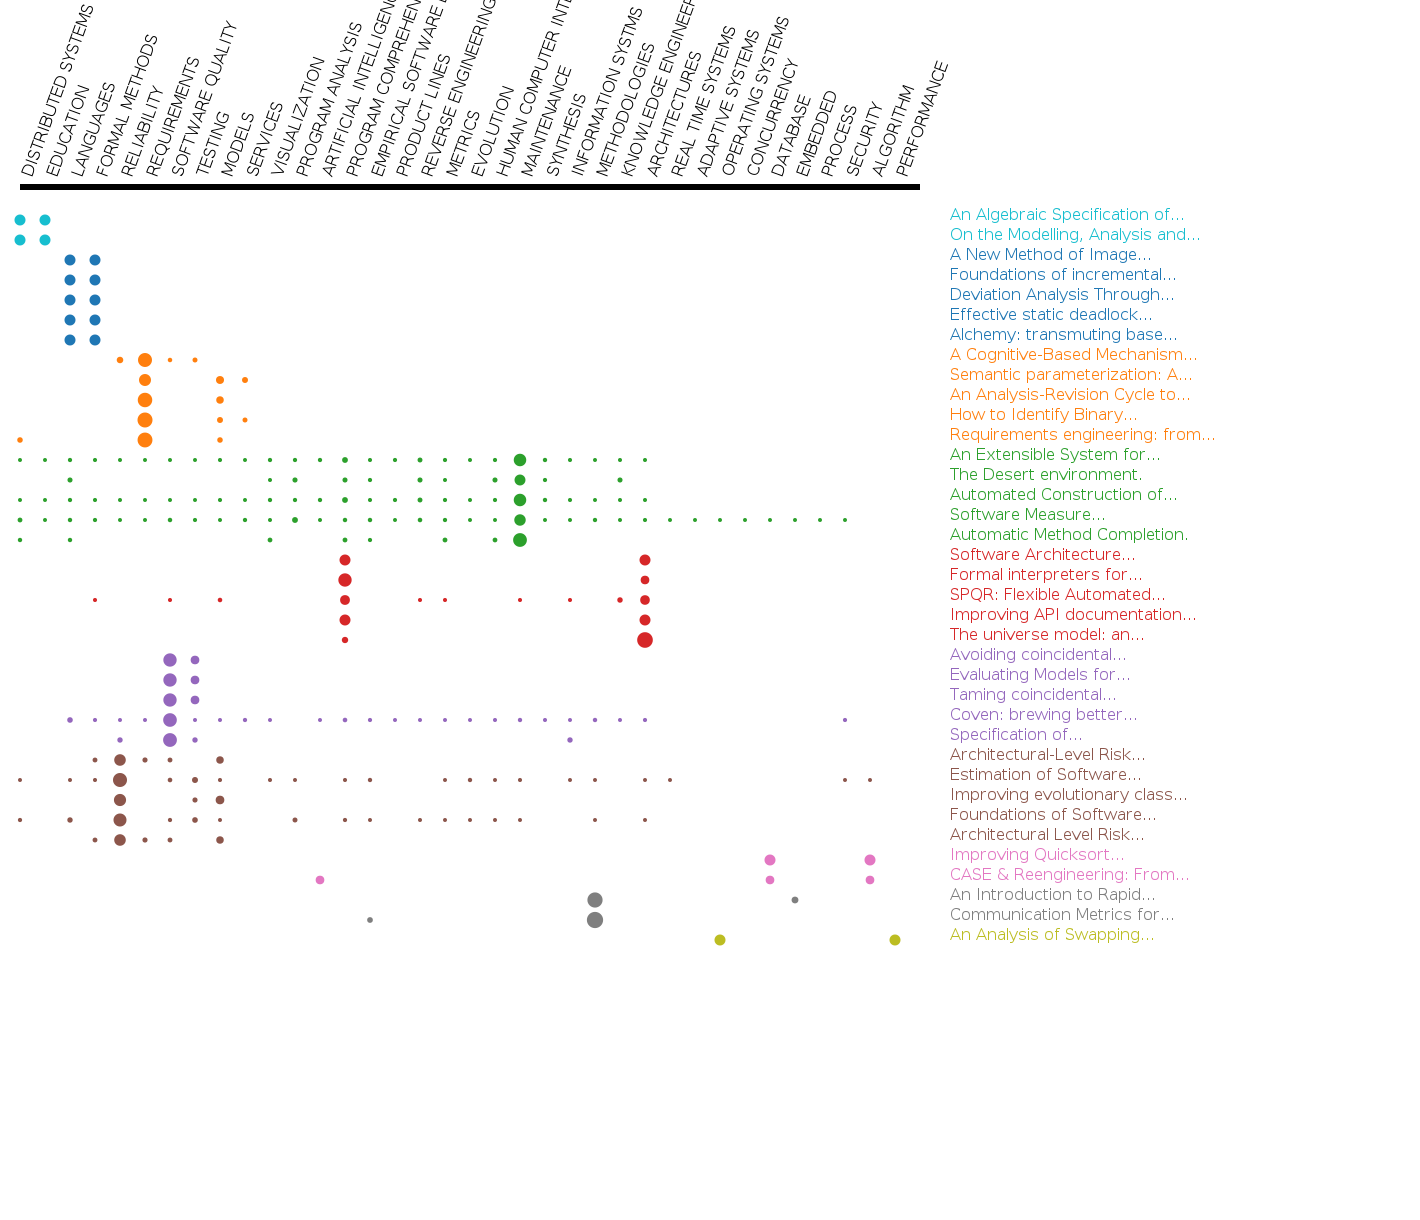
\includegraphics[width=0.8\textwidth]{resultados/papers/HAC/INTRA_INTER/gamma-01.png}
  \caption{Distribución de los perfiles por artículo y paquete $\gamma$ = $0.1$ y HAC - Intra Inter}
  \label{res:img-papers-gamma01-hac-intra-inter}
\end{figure}

\begin{figure}[H]
  \centering
    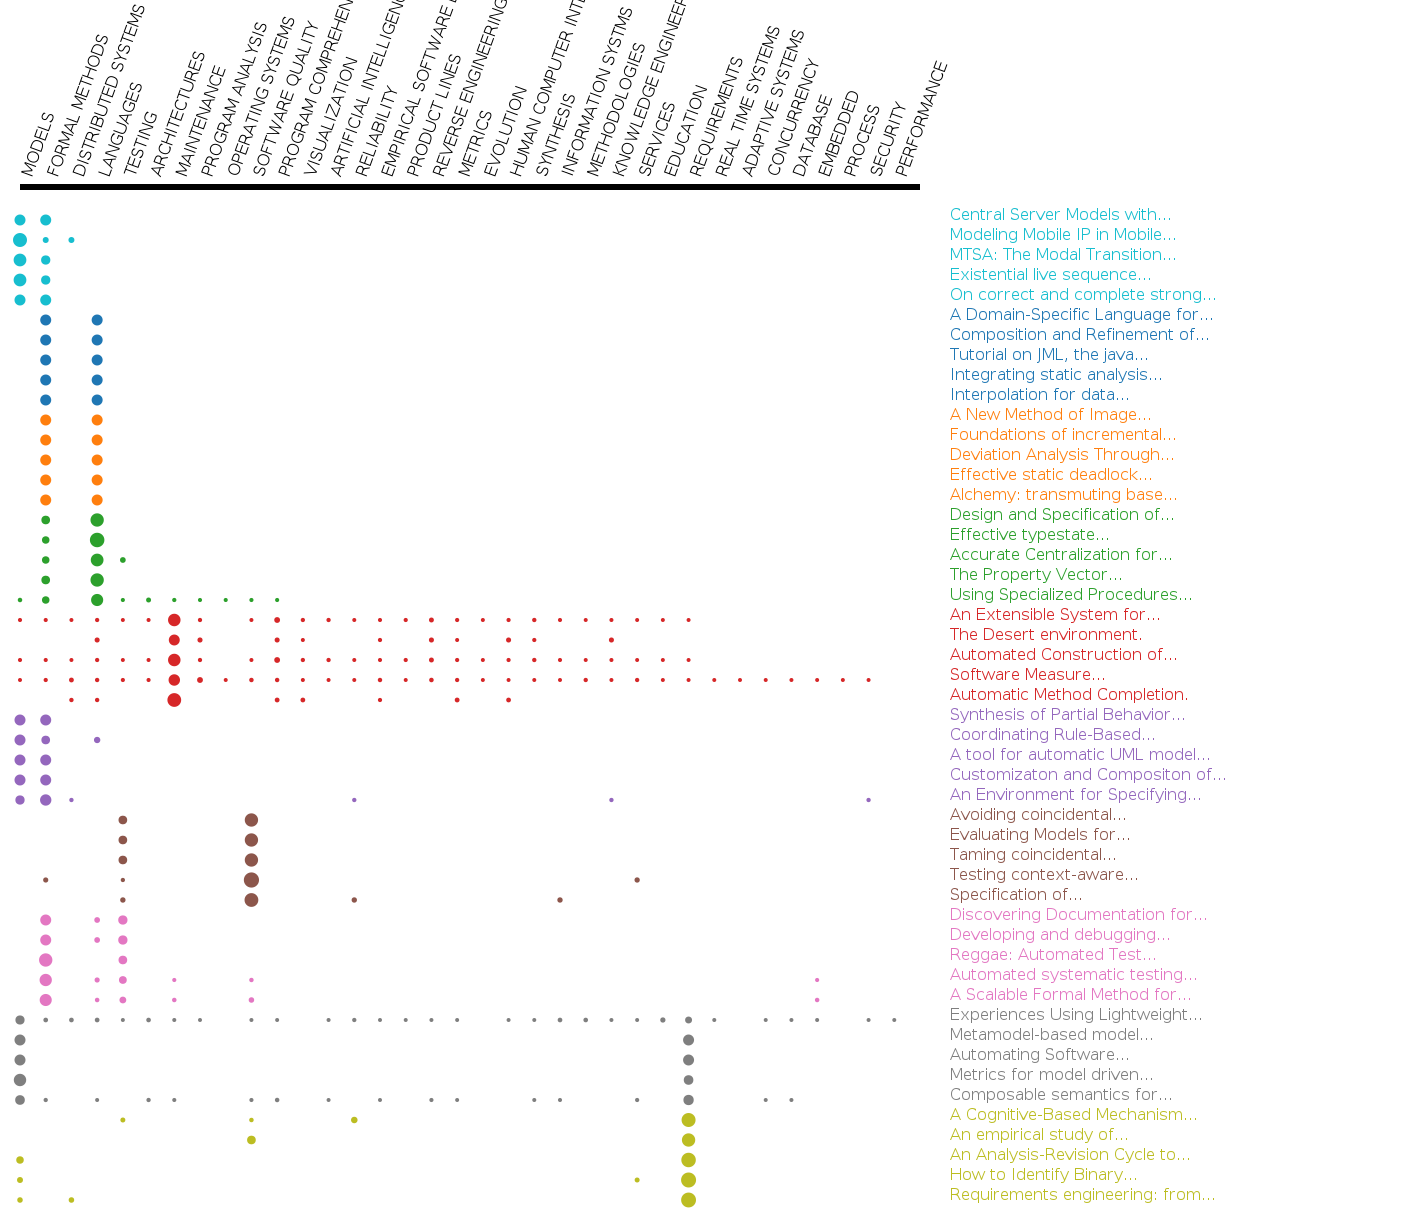
\includegraphics[width=0.8\textwidth]{resultados/papers/HAC/INTRA_INTER/gamma-09.png}
  \caption{Distribución de los perfiles por artículo y paquete $\gamma$ = $0.9$ y HAC - Intra Inter}
  \label{res:img-papers-gamma09-hac-intra-inter}
\end{figure}

\begin{figure}[H]
  \centering
    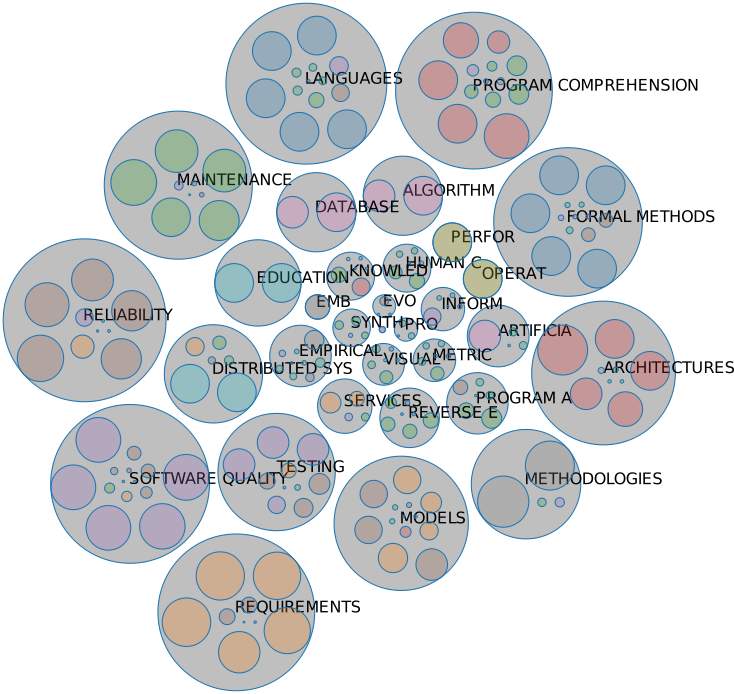
\includegraphics[width=0.8\textwidth]{resultados/papers/HAC/INTRA_INTER/bubbles-gamma-01.png}
  \caption{Distribución de los artículos por perfil $\gamma$ = $0.1$ y HAC - Intra Inter}
  \label{res:img-papers-bubbles-gamma01-hac-intra-inter}
\end{figure}

\begin{figure}[H]
  \centering
    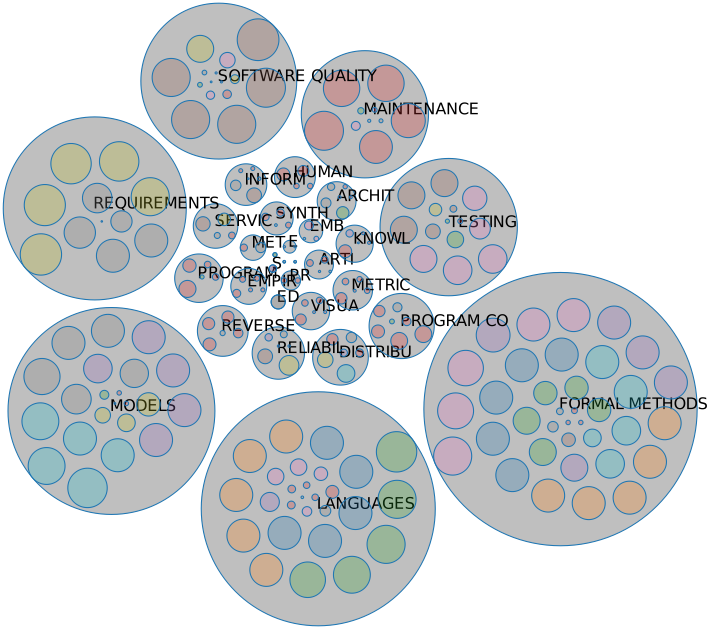
\includegraphics[width=0.8\textwidth]{resultados/papers/HAC/INTRA_INTER/bubbles-gamma-09.png}
  \caption{Distribución de los papers por perfil $\gamma$ = $0.9$ y HAC - Intra Inter}
  \label{res:img-papers-bubbles-gamma09-hac-intra-inter}
\end{figure}

De los gráficos \ref{res:img-papers-gamma01-hac-intra-inter} y \ref{res:img-papers-gamma09-hac-intra-inter} se observa que para $\gamma$ con valor cercano a cero, la solución contiene artículos con perfiles que cubren varios tópicos mientras que para $\gamma$ con valores más cercanos a uno, los tópicos de los artículos se concentran en unos pocos. Con esto se cumple el requerimiento de que cuando $\gamma$ se acerca el paquete es más cohesivo pero menos diverso (en \ref{res:img-papers-bubbles-gamma09-hac-intra-inter}. se observa la concentración de tópicos que hay en la solución).

Este comportamiento se repitió para todas las estrategias de selección que se utilizaron, la única diferencia fueron los valores finales de la función objetivo.
\paragraph{BOBO-100}
En este caso al ser muy grande la diferencia entre la utilización de la heurística Tabú y la ejecución sin ella,  se incluyó la misma para poder visualizar los cambios en la solución.
\begin{figure}[H]
  \centering
    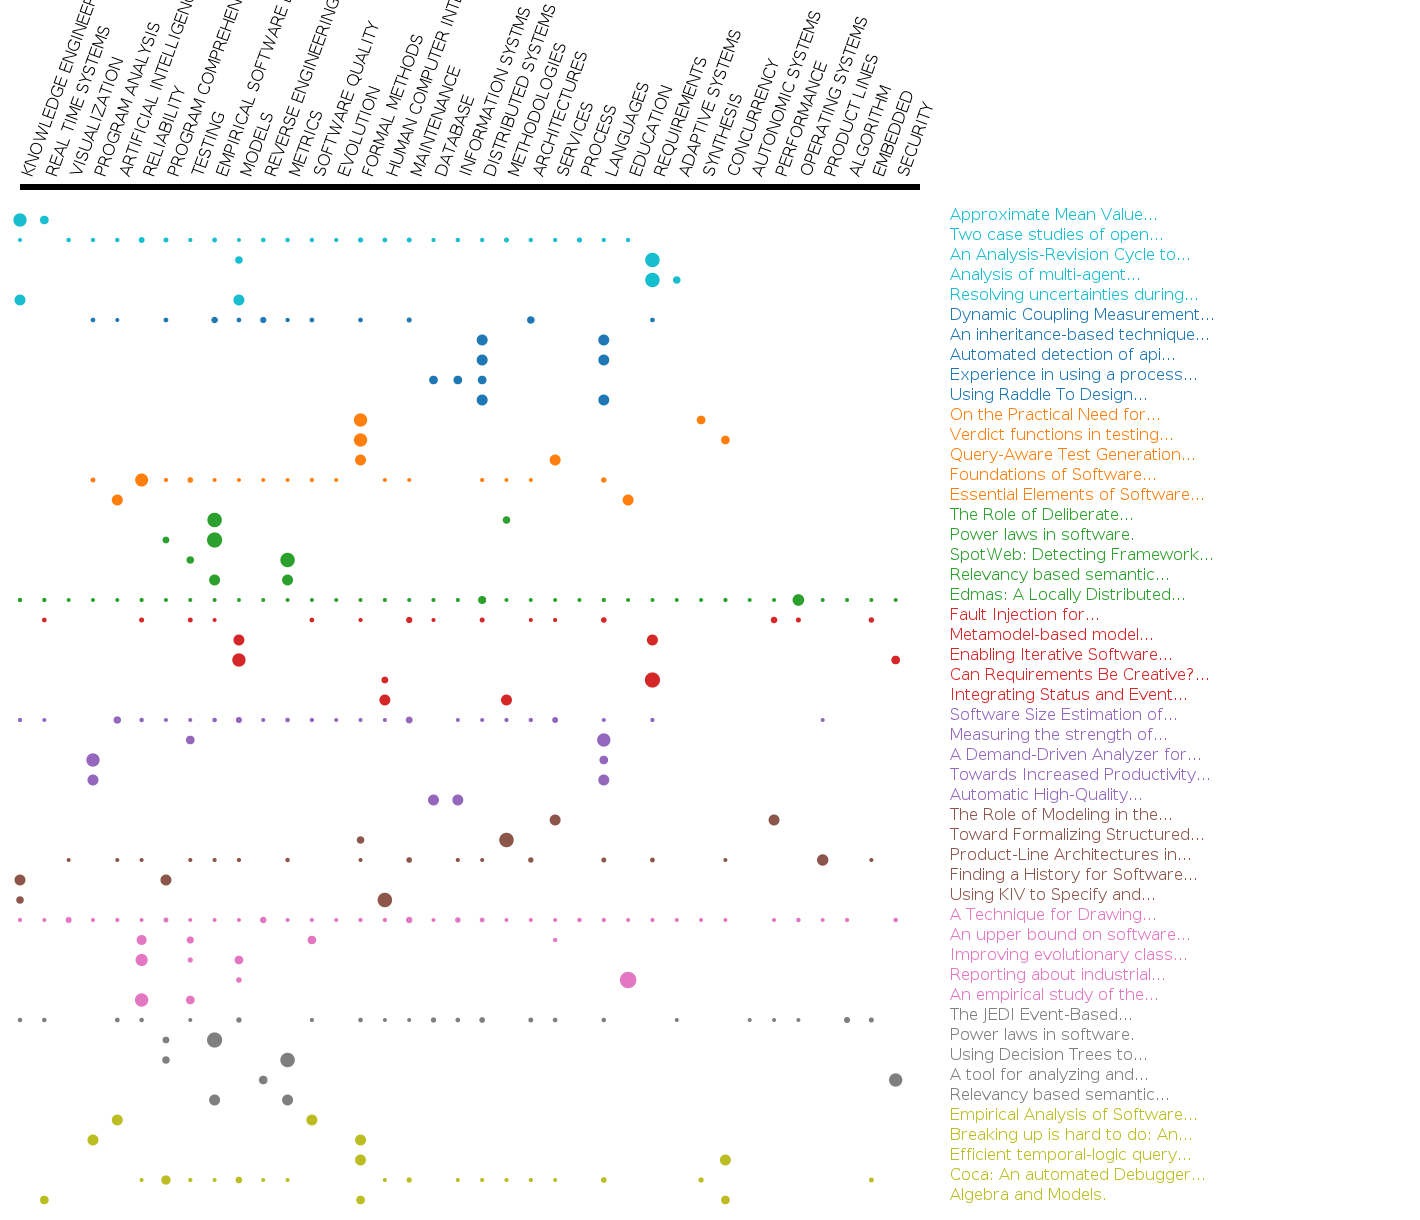
\includegraphics[width=0.8\textwidth]{resultados/papers/BOBO/INTRA_INTER/gamma-01.png}
  \caption{Distribución de los perfiles por artículo y paquete $\gamma$ = $0.1$ y BOBO - Intra Inter}
  \label{res:img-papers-gamma01-bobo-intra-inter}
\end{figure}

\begin{figure}[H]
  \centering
    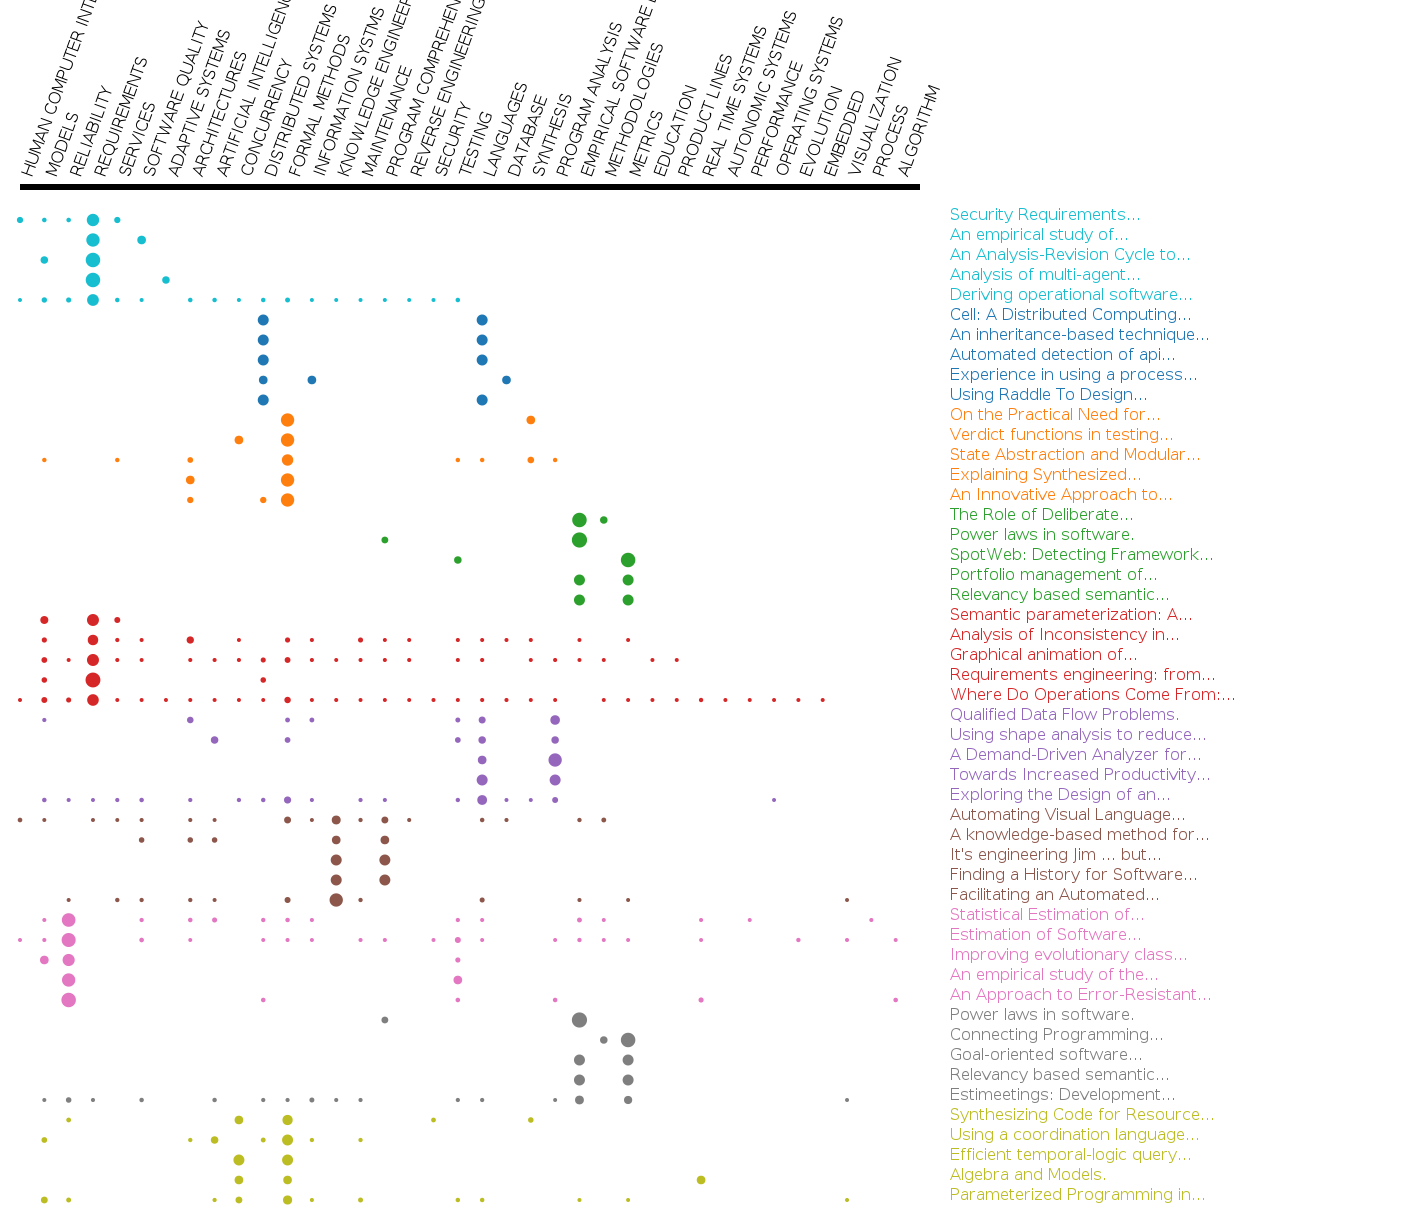
\includegraphics[width=0.8\textwidth]{resultados/papers/BOBO/INTRA_INTER/gamma-with-local-01.png}
  \caption{Distribución de los perfiles por artículo y paquete $\gamma$ = $0.1$ y BOBO - Intra Inter con búsqueda Tabú}
  \label{res:img-papers-gamma01-bobo-intra-inter-tabu}
\end{figure}

\begin{figure}[H]
  \centering
    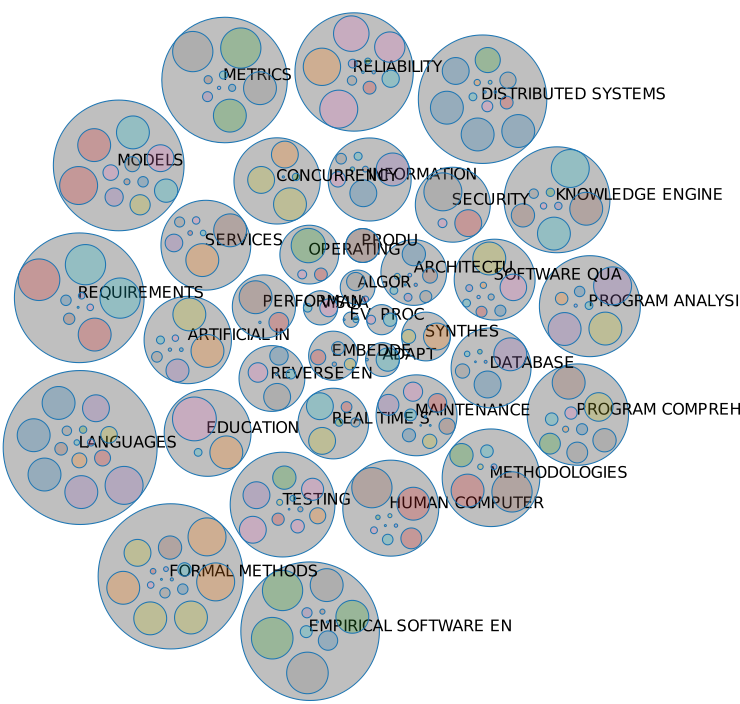
\includegraphics[width=0.8\textwidth]{resultados/papers/BOBO/INTRA_INTER/bubbles-gamma-01.png}
  \caption{Distribución de los artículos por perfil $\gamma$ = $0.1$ y BOBO - Intra Inter}
  \label{res:img-papers-bubbles-gamma01-bobo-intra-inter}
\end{figure}

\begin{figure}[H]
  \centering
    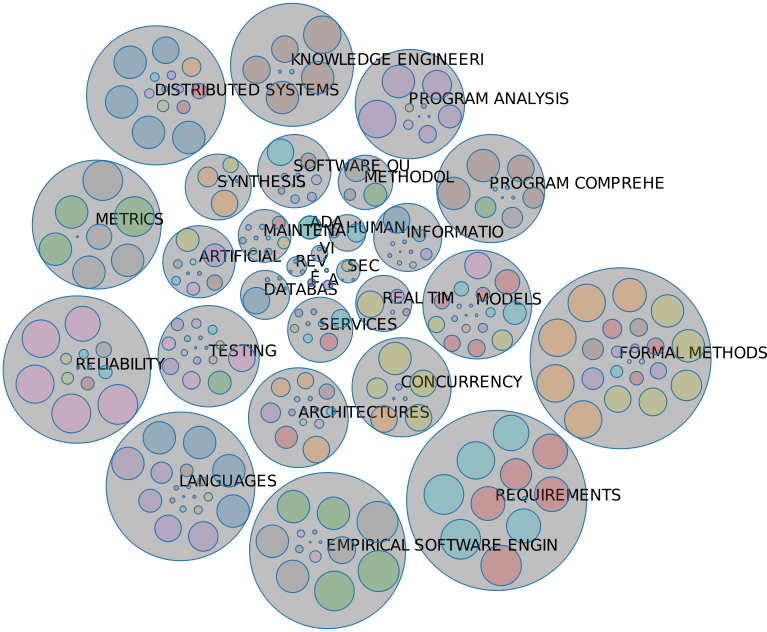
\includegraphics[width=0.8\textwidth]{resultados/papers/BOBO/INTRA_INTER/bubbles-gamma-with-local-01.png}
  \caption{Distribución de los artículos por perfil $\gamma$ = $0.1$ y BOBO - Intra Inter con búsqueda Tabú}
  \label{res:img-papers-bubbles-gamma01-hac-intra-inter-bobo}
\end{figure}

\begin{figure}[H]
  \centering
    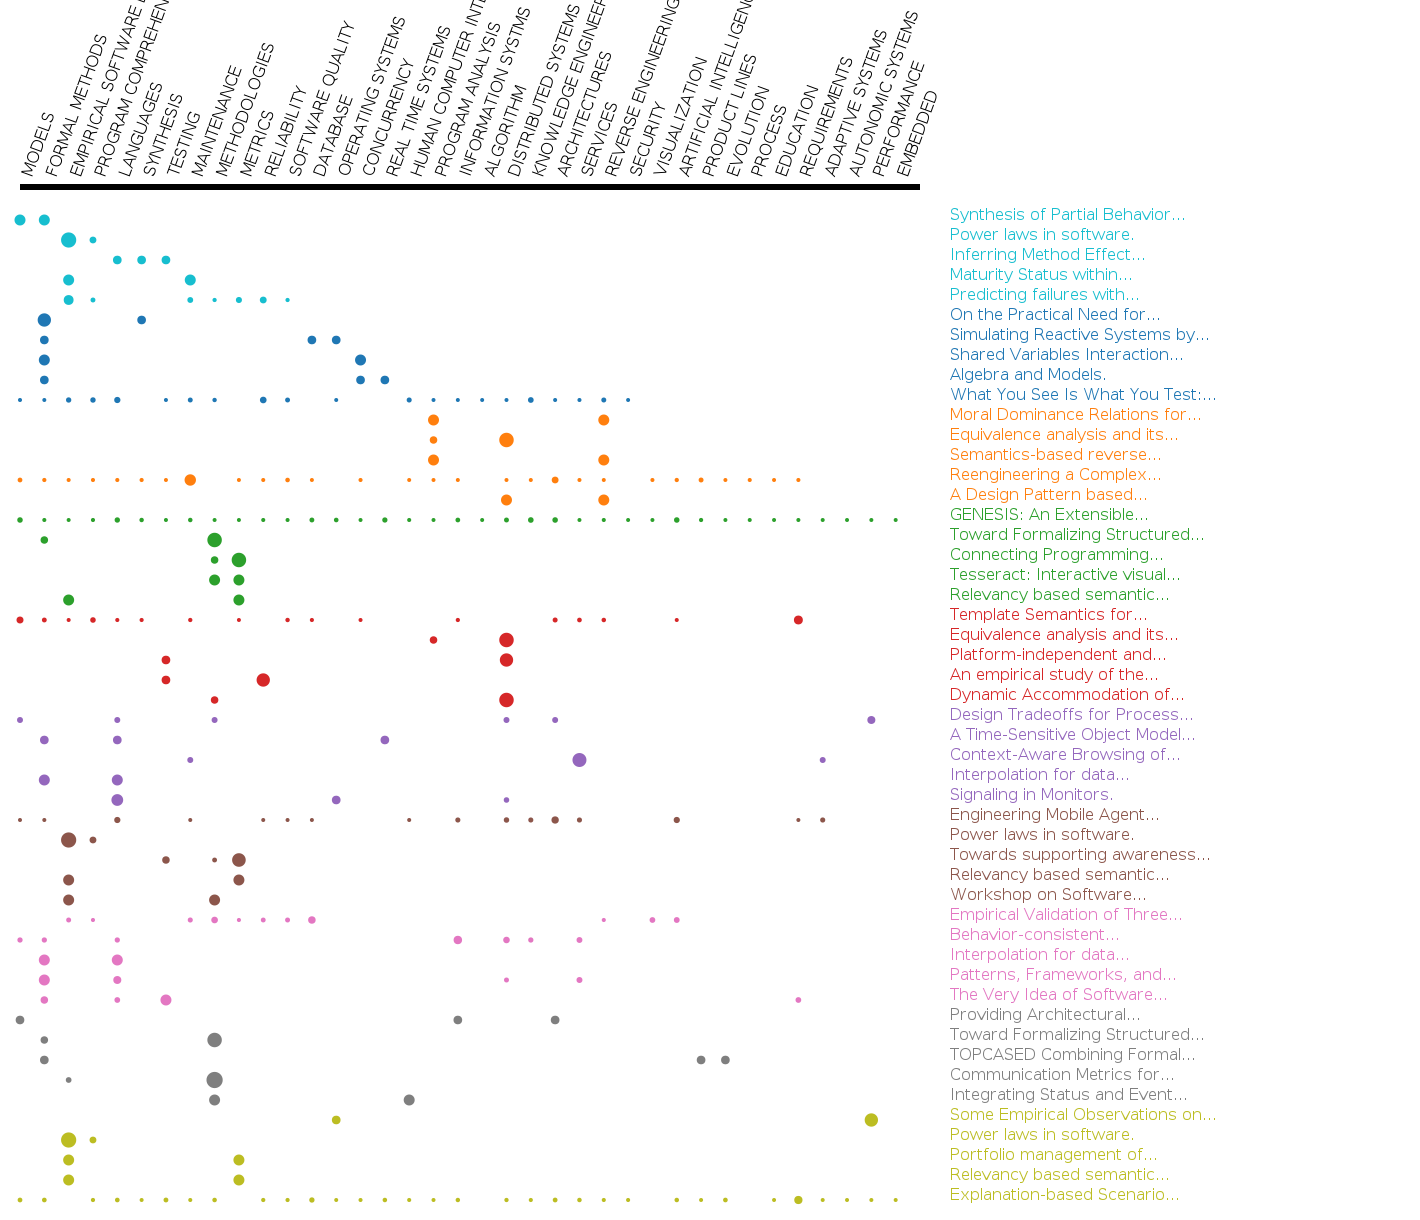
\includegraphics[width=0.8\textwidth]{resultados/papers/BOBO/INTRA_INTER/gamma-09.png}
  \caption{Distribución de los perfiles por artículo y paquete $\gamma$ = $0.9$ y BOBO - Intra Inter}
  \label{res:img-papers-gamma09-bobo-intra-inter}
\end{figure}

\begin{figure}[H]
  \centering
    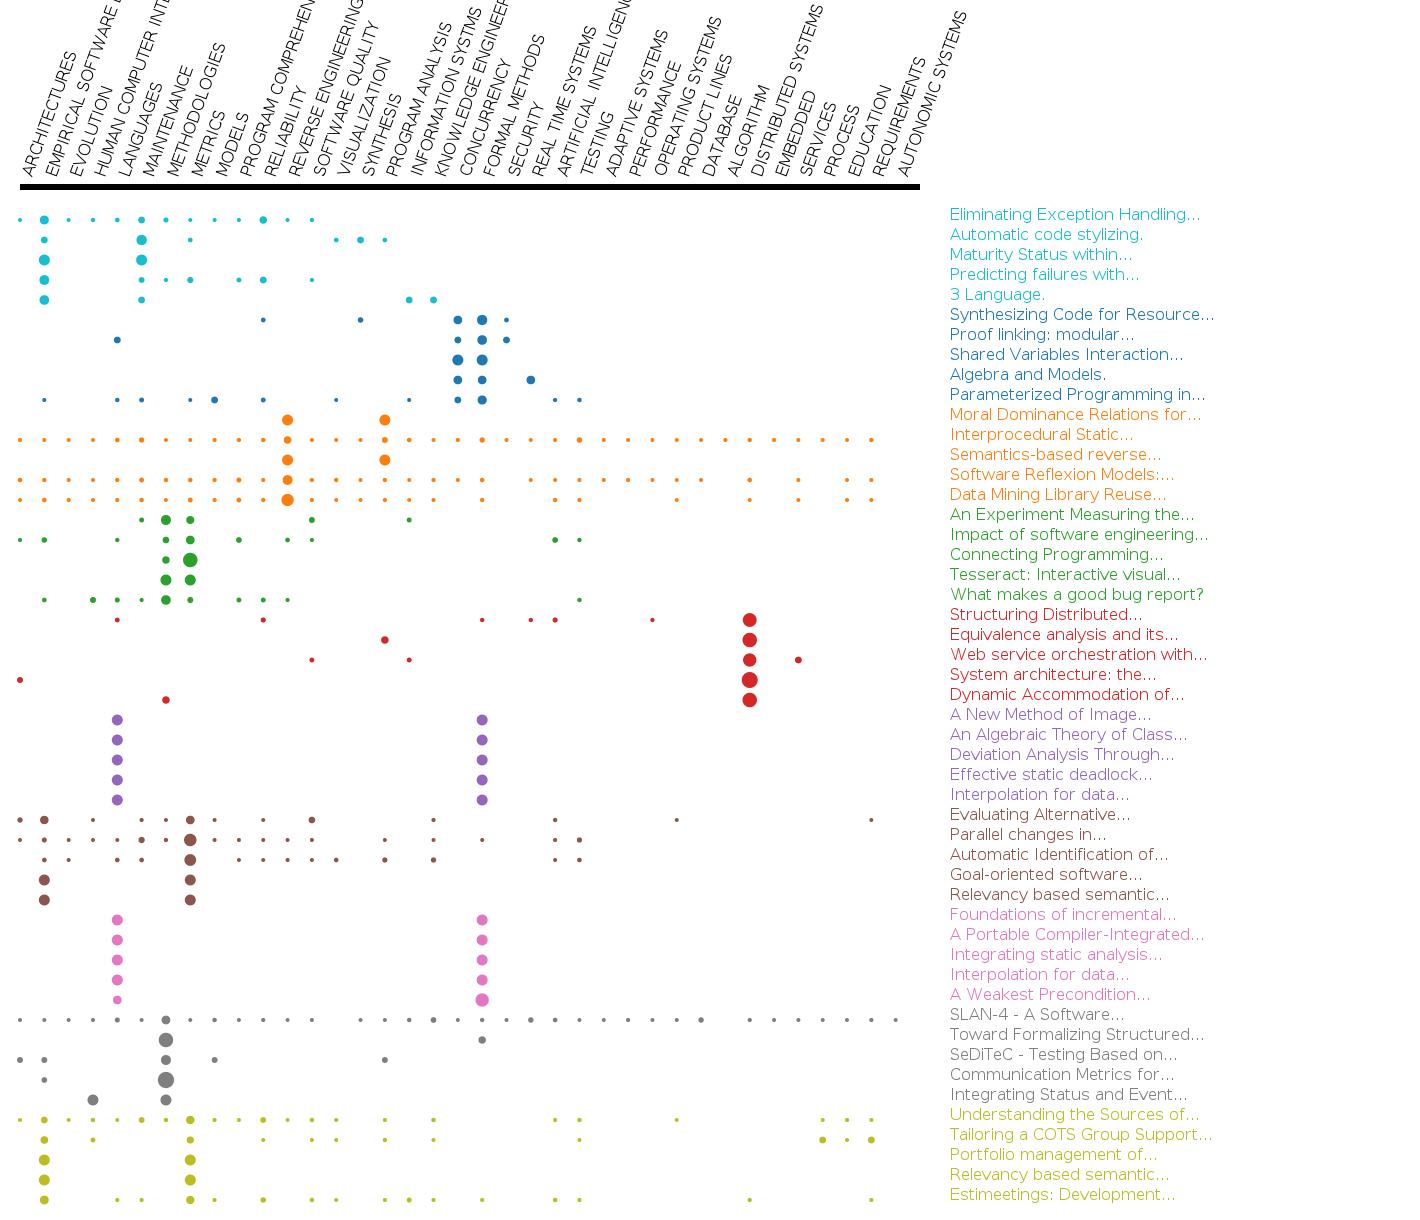
\includegraphics[width=0.8\textwidth]{resultados/papers/BOBO/INTRA_INTER/gamma-with-local-09.png}
  \caption{Distribución de los perfiles por artículo y paquete $\gamma$ = $0.9$ y BOBO - Intra Inter con búsqueda Tabú}
  \label{res:img-papers-gamma09-bobo-intra-inter-tabu}
\end{figure}

\begin{figure}[H]
  \centering
    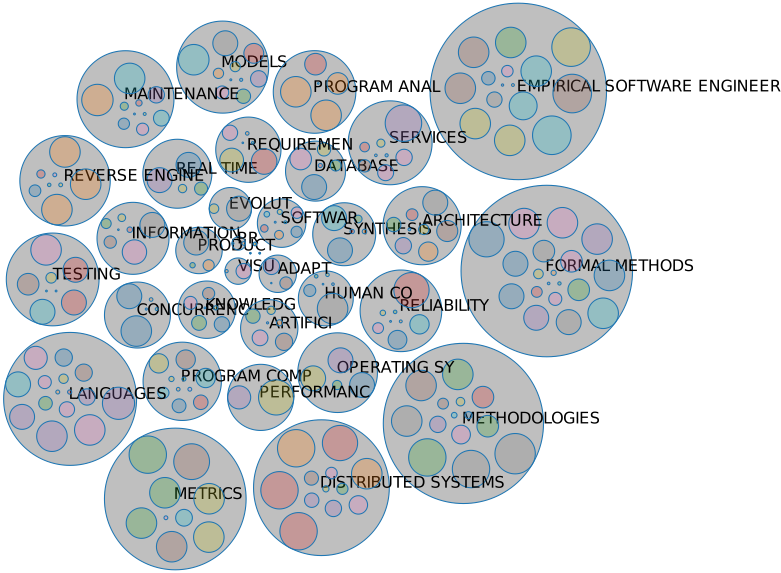
\includegraphics[width=0.8\textwidth]{resultados/papers/BOBO/INTRA_INTER/bubbles-gamma-09.png}
  \caption{Distribución de los artículos por perfil $\gamma$ = $0.9$ y BOBO - Intra Inter}
  \label{res:img-papers-bubbles-gamma09-bobo-intra-inter}
\end{figure}

\begin{figure}[H]
  \centering
    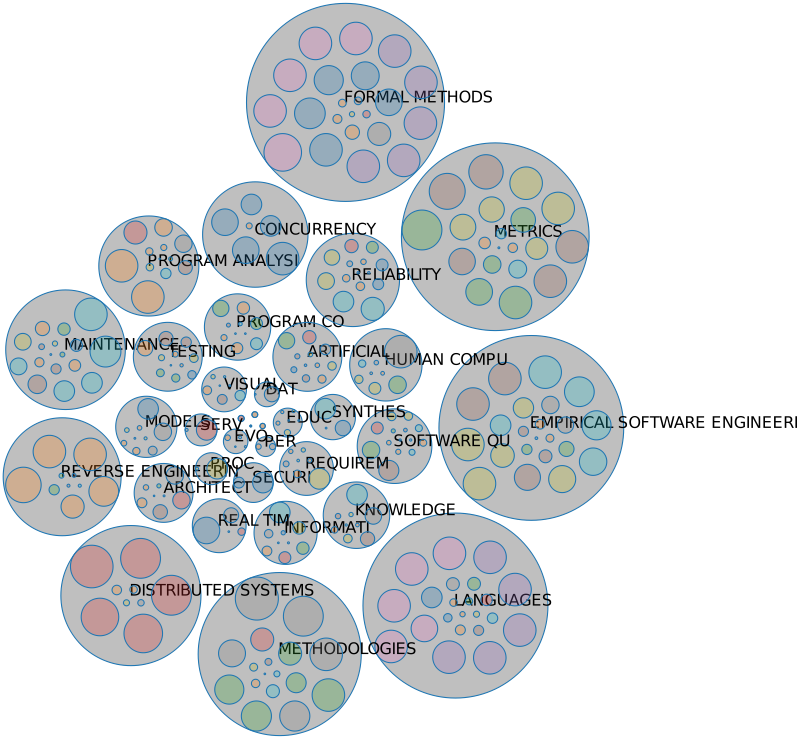
\includegraphics[width=0.8\textwidth]{resultados/papers/BOBO/INTRA_INTER/bubbles-gamma-with-local-09.png}
  \caption{Distribución de los artículos por perfil $\gamma$ = $0.9$ y BOBO - Intra Inter con búsqueda Tabú}
  \label{res:img-papers-bubbles-gamma09-hac-intra-inter-bobo}
\end{figure}
\newpage
\subsection{Búsqueda de Autores}
Solución de paquetes en el que cada uno contiene autores que escribieron artículos de tópicos similares y pertenecen a distinta universidad.

\begin{itemize}
  \item \textbf{Similitud}: Función que compara el perfil de los autores.
  \item \textbf{Complementariedad}: Universidad de pertenencia del autor.
\end{itemize}

La instancia elegida, luego de la depuración, cuenta con $5577$ autores en condiciones de ser elegidos por los algoritmos implementados.

\begin{figure}[H]
  \centering
    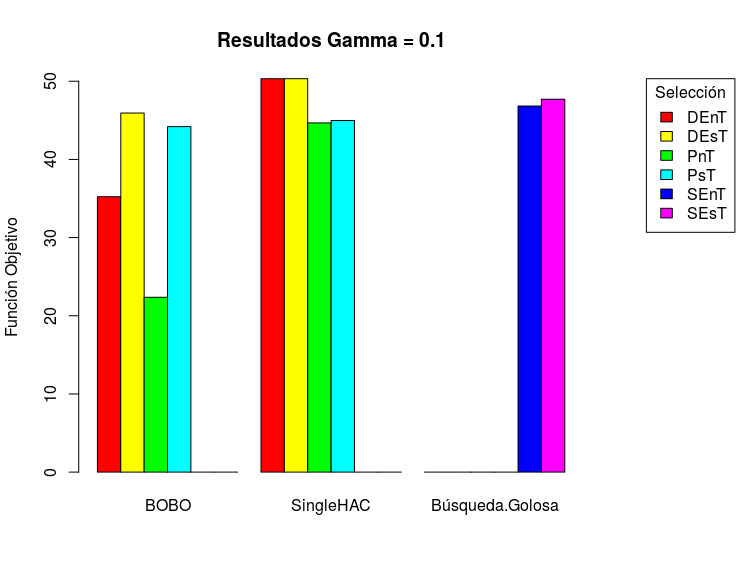
\includegraphics[width=0.8\textwidth]{resultados/authors/Graficos_agrupados/gamma01-autores.png}
  \caption{Función Objetivo $\gamma$ = $0.1$ vs Algoritmos de resolución}
  \label{res:img-autores-agr-gamma01}
\end{figure}

\begin{figure}[H]
  \centering
    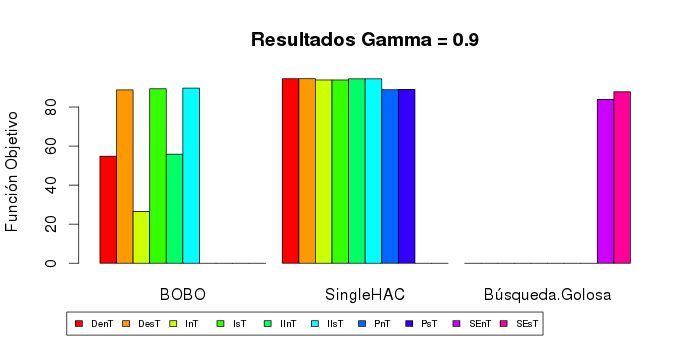
\includegraphics[width=0.8\textwidth]{resultados/authors/Graficos_agrupados/gamma09-autores.png}
  \caption{Función Objetivo $\gamma$ = $0.9$ vs Algoritmos de resolución}
  \label{res:img-autores-agr-gamma09}
\end{figure}

El comportamiento de las ejecuciones fueron muy similares a las que se obtuvieron en la búsqueda de artículos. La utilización de la Búsqueda Tabú mejoró sustancialmente el algoritmo \texttt{BOBO} en todos sus variantes. En el caso de \texttt{Efficient - HAC}, solo mejoró con la estrategia de selección \texttt{Proportional}. Casualmente fue la única estrategia que tuvo un comportamiento diferente en relación a la búsqueda de artículos, en la cuál la función objetivo siempre tuvo valores mayores o iguales a por ejemplo la selección \texttt{INTRA} y en este caso fue menor o igual. Igualmente las diferencias en términos de valor son mínimas que se deben a la conformación de los perfiles de los elementos.

Como se menciona anteriormente, al no comportarse de una manera diferente a la búsqueda de artículos no se incluyeron los gráficos.
\newpage
\subsection{Búsqueda de universidades}\label{res:busInstituciones}
Solución de paquetes en el que cada uno contiene universidades de distintas regiones en las que se escribieron artículos de tópicos.
\begin{itemize}
  \item \textbf{Similitud}: Función que compara el perfil de las instituciones.
  \item \textbf{Complementariedad}: Región a la que pertence la instituciones.
\end{itemize}

\begin{figure}[H]
  \centering
    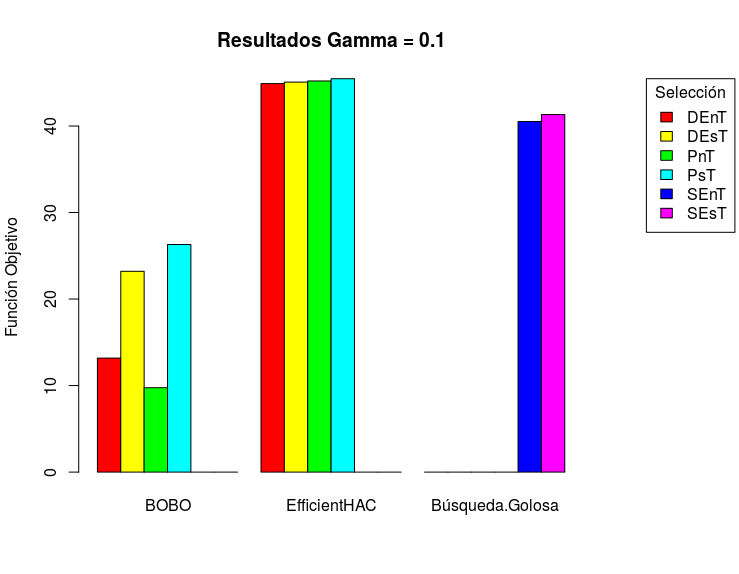
\includegraphics[width=0.8\textwidth]{resultados/affiliations/Graficos_agrupados/gamma01-affiliations.png}
  \caption{Función Objetivo $\gamma$ = $0.1$ vs Algoritmos de resolución}
  \label{res:img-affiliations-agr-gamma01}
\end{figure}

\begin{figure}[H]
  \centering
    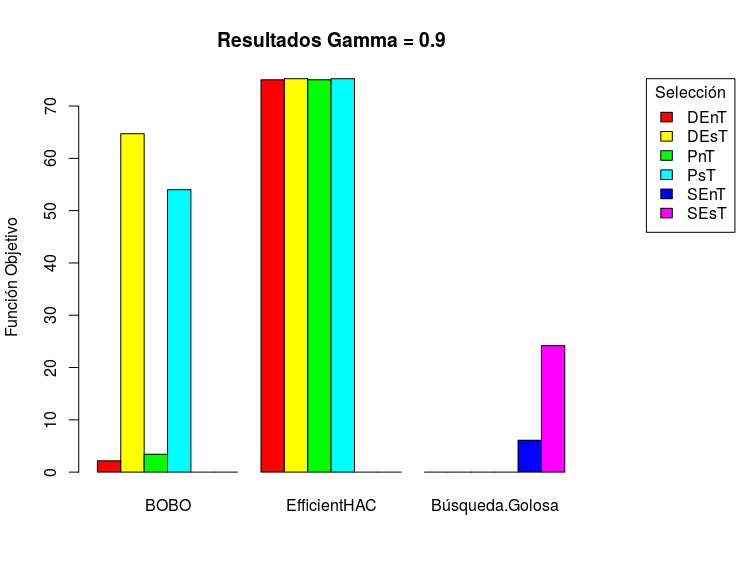
\includegraphics[width=0.8\textwidth]{resultados/affiliations/Graficos_agrupados/gamma09-affiliations.png}
  \caption{Función Objetivo $\gamma$ = $0.9$ vs Algoritmos de resolución}
  \label{res:img-affiliations-agr-gamma09}
\end{figure}

Como se observa en los gráficos anteriores el uso de las búsquedas Tabú siempre mejora la solución obtenida en primer lugar, sin importar que algoritmo se haya utilizado previamente. Particularmente, y al igual que en los demás experimentos, la variante \texttt{BOBO} es siempre la más beneficiada por el uso de la metaheurística ya que el valor de la función objetivo de la solución final por lo menos duplica al correspondiente de la solución original.

A diferencia de los escenarios anteriores el algoritmo \texttt{Goloso} para $\gamma\ =\ 0.9$ no obtuvo resultados buenos como se esperaba.
\newpage
\section{Búsqueda de atracciones turísticas}\label{res:busAtracciones}
Los resultados son conjuntos de paquetes que cada uno contiene atracciones turísticas de distinta temática, que son similares con respecto a la distancia geográfica y la suma del precio de las atracciones no supera el presupuesto.
\begin{itemize}
  \item \textbf{Similitud}: Cercanía geográfica de las atracciones.
  \item \textbf{Complementariedad}: Tipo de atracción turística.
  \item \textbf{presupuesto}: Cantidad de dinero que tiene el usuario para utilizar.
\end{itemize}
Se generaron soluciones con las siguientes características:\\

\SolucionBudget
{}
{
\begin{description}
	\item[alg\_1] \texttt{Búsqueda Golosa}
	\item[alg\_2] \texttt{PAC(BOBO-100/Selección de paquetes proporcional)}
	\item[alg\_3] \texttt{PAC(BOBO-100/Selección de paquetes)}
	\item[alg\_4] \texttt{PAC(Efficient C-HAC/Selección de paquetes proporcional)}
	\item[alg\_5] \texttt{PAC(Efficient C-HAC/Selección de paquetes)}
\end{description}
}
{$(0,1; 0,3; 0,5; 0,7; 0,9)$}
{10}
{3}
{7}

\begin{figure}[H]
  \centering
    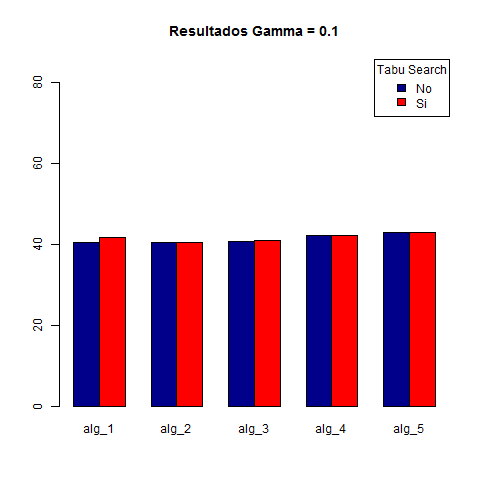
\includegraphics[width=0.8\textwidth]{resultados/cities/Graficos_agrupados/gamma01-cities.png}
  \caption{Función Objetivo $\gamma$ = $0.1$ vs Algoritmos de resolución}
  \label{res:img-cities-agr-gamma01}
\end{figure}

\begin{figure}[H]
  \centering
    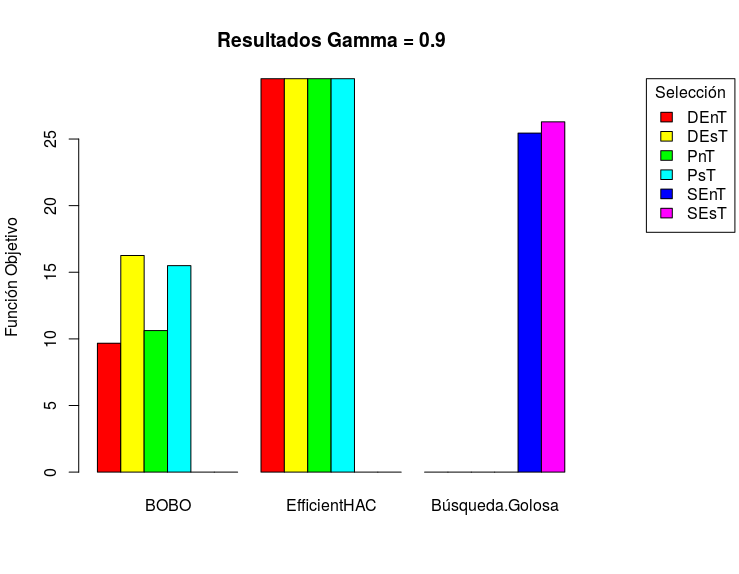
\includegraphics[width=0.8\textwidth]{resultados/cities/Graficos_agrupados/gamma09-cities.png}
  \caption{Función Objetivo $\gamma$ = $0.9$ vs Algoritmos de resolución}
  \label{res:img-cities-agr-gamma09}
\end{figure}

En esta instancia se repite el comportamiento de los resultados obtenidos en las consultas realizadas sobre la base de datos de artículos. La solución del algoritmo goloso supera al de PAC cuando la estrategia de producción es con BOBO pero con HAC valor de la función objetivo es similar. También, en esta instancia, se obtuvieron mejores valores con la selección proporcional.

Al aplicar la búsqueda tabú se mejora sustancialmente la solución obtenida con PAC con la estrategia BOBO, obteniendo una solución tan optima como con el resto de los algoritmos. Con el resto de los algoritmos no se obtiene una mejora sustancial de la solución al aplicar la búsqueda tabú.

Solo se muestran los gráficos y comportamientos para las pruebas realizadas con un solo presupuesto, pero los mismos tuvieron el mismo efecto a medida que se cambiaba ese valor.
